\subsection{Sprint 4: Using real money}
In this sprint, we will focus on our final feature.
The last major challenge remaining at this point was linking the virtual marketplace to the real world.
So far, users can trade their digital commodities for any amount of virtual currency.
The problem was that this currency had no actual value, since the only way of obtaining it was by trading it for reputation points.
So the marketplace at this point would consist of people selling reputation points and others that do not have the means to acquire their own points, trying to buy them.
However, without any value attached to this virtual currency, no incentive is given to start trading.
The solution to this problem is to allow users to use real money to either buy virtual currency or use that money directly in the transaction.

\subsubsection{Usage of virtual currency}
Virtual currency is a great way to keep the identities of users hidden when making financial transactions. 
The problem with this structure is that it requires a way to verify whether the digital money is actually real and not spoofed. 
Without a central authority that governs all transactions, it becomes very difficult to tell whether or not the digital money is legitimate.
Of course, there are solutions.

For example, one could implement a block-chain structure like BitCoin has made \cite{bitcoin}.
With this, the whole user-base has to agree on a certain chain of transactions.
To achieve this, it is required to have every user communicate with every other user what transactions are made.
This method of regular broadcasting does not scale and is the reason Tsukiji switched to a gossip model.

The solution for Tsukiji was to abandon the idea of virtual currency altogether.
If users can use existing payment options, we no longer have to worry about security en legitimacy issues that payments bring.
All that is required of Tsukiji is to link one peer to another peer and facilitate an easy way to perform the transaction.
The privacy issue is now brought back to the user.
If they desire anonymous transactions, they will have to ensure this themselves with their preferred payment option.

\subsubsection{Online banking}
In order to use real money, we required a third party to handle payments for us. 
After some research, two options had our preference: iDeal and Paypal.
Sadly, the iDeal API had the constraint that it only allowed users to give money to businesses and did not facilitate payments from person to person.
This would mean that every user has to create a business account and have it approved by iDeal, just to make payments in Tsukiji.
As this is not deemed feasible, we chose to use Paypal instead.
\begin{figure}[H]
  \centering
  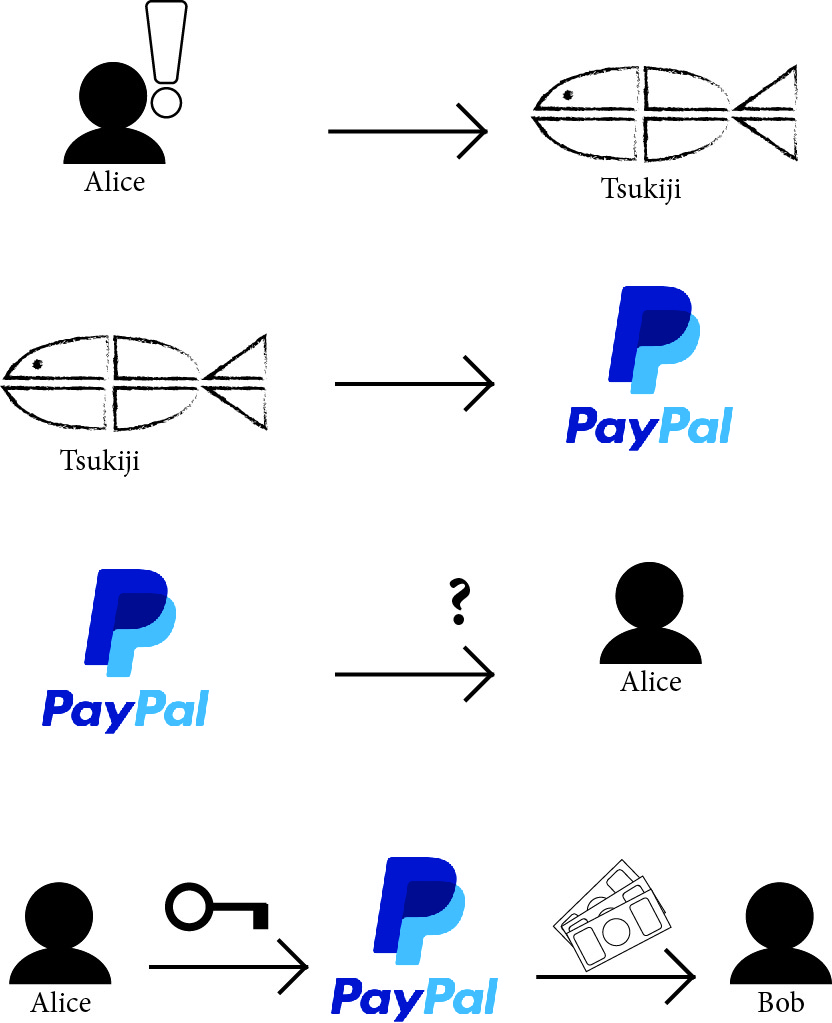
\includegraphics[width=\linewidth]{paypal-payment}
  \caption{Alice finds an interesting item on Tsukiji. Tsukiji then aks the PayPal API to create an authorisation page. This page asks Alice for her login details and then verifies the transaction, sending the money from Alice's paypal account to Bob's.}
  \label{paypal_pay}
\end{figure}

\newpage
The Paypal API \cite{paypal} offers many ways to create, send and verify transactions.
While poorly documented, there is a python integration suite that uses http calls with JSON objects to communicate with the Paypal servers.
The current implementation in Tsukiji creates a payment page when a trade is made.
The page has the amount (in euros) and the recipient pre-filled.
All the user has to do now is login on the Paypal website and authorise the transaction.

The full process is depicted in Figure \ref{paypal_pay}.
This way the user does not need to trust Tsukiji with their Paypal credentials and does not even need to know the address of the person they are about to pay.
This approach keeps Tsukiji decentralised as well, since the Paypal service is not part of the implementation of Tsukiji itself.
It should still be possible to equip Tsukiji with different payment options.

Tsukiji now has a way for users to pay each other that is reliable but leaves itself unaccountable for any errors in transactions.
Users only have to trust Paypal for their transactions, which complies with the zero-trust ideology of a decentralised system.
